\documentclass[a4paper, 10pt]{article}
\usepackage[a4paper, total={6in, 10in}]{geometry}
\usepackage[printsolution=false]{exercises}
\usepackage{url}
\usepackage{background, hyperref}
\usepackage{tcolorbox}
\usepackage{float}
\usepackage{lastpage}
\usepackage{fancyhdr}
\usepackage{xcolor}
\usepackage[sfdefault]{cabin}
\usepackage{graphicx}
\usepackage{wrapfig}
\usepackage[T1]{fontenc}
\usepackage[backend=bibtex,style=authoryear,natbib=true, maxbibnames=9, maxcitenames=2]{biblatex}
\bibliography{howeetal18.bib}
\usepackage{todonotes}
%\bibliographystyle{besjournals}
\setlength\parindent{0pt}
\pagestyle{fancy}
\fancyhead[L,C,R]{}
\fancyfoot[L]{\small CTDS workshop, Univ. of St Andrews}
\fancyfoot[R]{\small Practical 4 - model selection}
\fancyfoot[C]{\small \thepage\ of \pageref{LastPage}}
\renewcommand{\headrulewidth}{0pt}
\renewcommand{\footrulewidth}{1pt}

\newif\iffirstpage
\firstpagetrue
\backgroundsetup{contents={%
 			\iffirstpage
				\includegraphics[width=\textwidth]{jaguar1.jpg}%
				\global\firstpagefalse
				\fi
			},
			scale=1,placement=top,opacity=0.6,position=current page.north, vshift=-1cm
}

\begin{document}
%% don't mess with blank lines here in the title.
\phantom{a}

\vspace{4.7cm}

{\Large Camera trap distance sampling workshop}

{\large 21-25 March 2022}

\begin{flushright}
\tiny{Source: \url{https://unsplash.com/@satyadeep_d}}
\end{flushright}

\ifsolutionthenelse{%
{\Large \color{blue}Solution \\}
{\color{blue}\rule{\linewidth}{0.5mm}}
}%
{%
}

Fundamental to sound inference regarding animal abundance from distance sampling analysis of camera trap data is selection of appropriate detection function models.  That process is made more difficult when analysing camera trap data because of the problem of overdisperson.  This practical demonstrates the process of model selection that copes with overdispersion.

\section{Model selection adjustments from overdispersion}

Overdispersion causes AIC to select overly-complex models, so analysts should specify the number/order of adjustment terms manually when fitting distance sampling models to data from camera traps, rather than allowing automated selection using AIC. \textcite{howe_model_2019} describes two methods for performing model selection of distance sampling models in the face of overdispersion.  The first method of \textcite{howe_model_2019} employs a two-step process and is implemented in the most recent version of Distance for Windows. 

\begin{wrapfigure}{r}{0.35\textwidth}
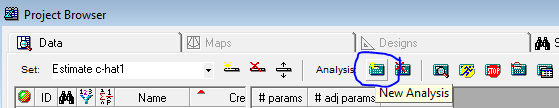
\includegraphics[width=0.33\textwidth]{images/new.png}
\caption{With the analysis of interest highlighted, press the \emph{New analysis} button to duplicate that analysis. \label{fig:newa}}
\vspace{-25pt}
\end{wrapfigure}

We will walk through the process of selecting the most appropriate model from the candidate model set you fitted in Practical 2.



\section{Step 1: compute $(\hat{c_1})$ for most complex key function models}

\begin{itemize}
	\item Open project used in Practical 2 to the analysis set you created in that practical.
	\item Create three additional columns using \emph{Column browser}
	\begin{itemize}
		\item GOF Chi2/df, c-hat and QAIC
		\begin{itemize}
			\item The difference between \textbf{GOF Chi2/df} and \textbf{c-hat}: \textbf{c-hat} is a user-supplied value, while \textbf{GOF Chi2/df} is a statistic computed for a fitted model.  You will copy the \textbf{GOF Chi2/df} from a fitted model and input it (Fig. \ref{fig:chat}) as \textbf{c-hat} into a model about to be fitted.
		\end{itemize}
	\end{itemize}
	\item Duplicate (using the \emph{New analysis} button, Fig. \ref{fig:newa} these analyses and run them again
		\begin{itemize}
			\item unicos 3, hncos 2, hrsimp 1
			\item these are the most complex models for each key function family
		\end{itemize}
	\item At this point, you will have 11 models in the analysis set; 8 from Practical 2 and the 3 models you duplicated and re-ran.
\end{itemize}

\ifsolutionthenelse{%
%	\begin{tcolorbox}[colback=green!5!white, colframe=green!60!black, title=Step 1]
\begin{figure}
	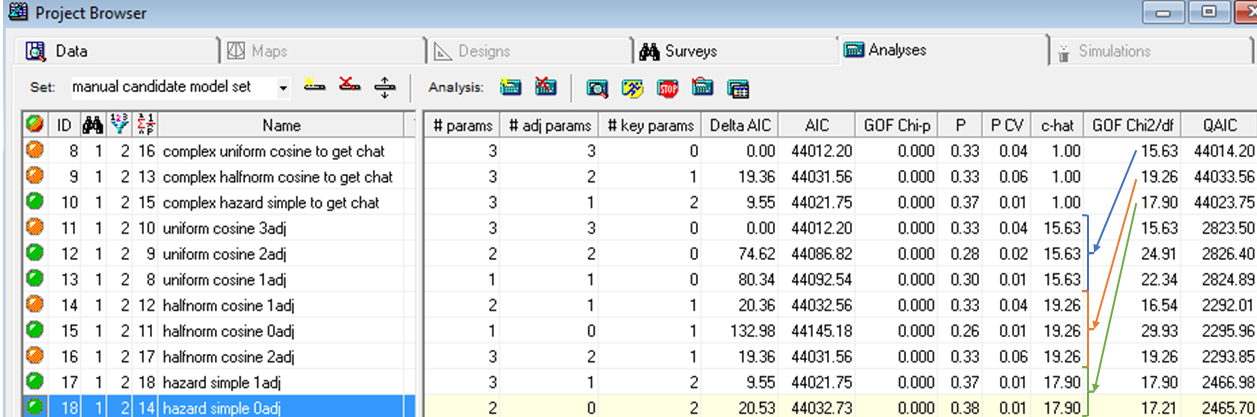
\includegraphics[width=\textwidth]{images/selection-steps-1.png}
\caption{Project browser after supplying $\hat{c_1}$ values to all candidate models and re-running them. Coloured lines show application of $\hat{c_1}$ values from complex model to all other models in key function family. \label{fig:step1}}
\end{figure} 
%\end{tcolorbox}
}
{
}


\begin{wrapfigure}{r}{0.35\textwidth}
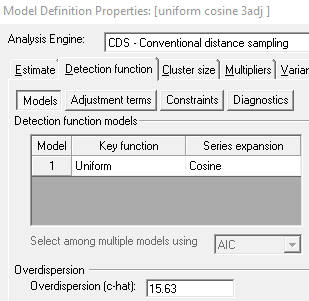
\includegraphics[width=0.33\textwidth]{images/chat-input.png}
\caption{Supplying $\hat{c_1}$ value for all candidate models. \label{fig:chat}}
\vspace{-25pt}
\end{wrapfigure}

\section{Step 2: compute QAIC for each of the 8 models}

Now that the values of $(\hat{c_1})$ are available after refitting the complex models, we will re-fit all 8 models of the candidate model set to produce QAIC values:
$$QAIC = -2 \left \{ \frac{log(\mathcal{L}(\hat{\theta}))}{\hat{c}} \right \} + 2K$$

\begin{itemize}
	\item Using the \emph{GOF Chi2/df} values, edit each of the 8 models previously fitted, inserting the \emph{GOF Chi2/df} for a key function family into the \emph{c-hat} field in the \emph{Model properties} page (Fig. \ref{fig:chat}) for all models in that key function family and refit.  The refit will over-write previous results; you will see the values in the QAIC and c-hat columns change to reflect the changes you made.
	\item For each key function family (uniform, half normal, hazard rate), examine the \textbf{QAIC} column for models in that family.  The model with the smallest QAIC is the preferred model from its respective family.
\end{itemize}


\ifsolutionthenelse{%
%	\begin{tcolorbox}[colback=green!5!white, colframe=green!60!black, title=Step 2]
\begin{figure} [H]
	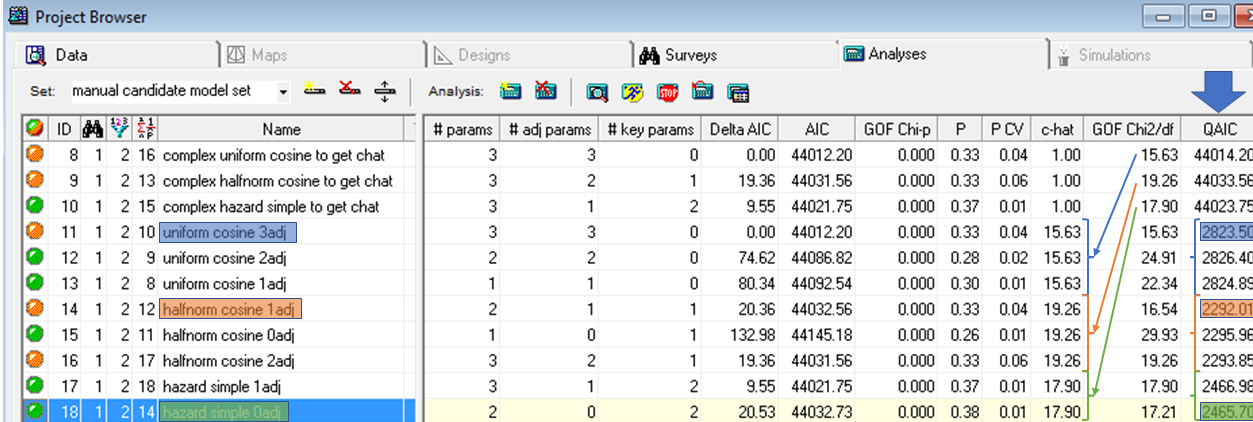
\includegraphics[width=\textwidth]{images/selection-steps-2.png}
\caption{Project browser following Step 2.  Emphasis is upon QAIC values within each key function family.  Smallest QAIC value within each key function family are highlighted in the QAIC column.  These models go forward to Step 3. \label{fig:step2}}
\end{figure} 
%\end{tcolorbox}
}
{
}

\section{Step 3: select best model from Step 2 champions}
The suite of candidate models has now been narrowed from 8 to 3 using the QAIC process from the previous step. 

The final stage in the model selection process is to examine the column of the \emph{Results Browser} containing \emph{GOF Chi2/df} values for the three models selected in the previous step.  The model to be used for inference for the duiker data set is the model with the smallest \emph{GOF Chi2/df} value.

With model selection complete, in the next practical, we will examine the density estimates produced from this model following adjustments that account for partial fields of camera view and temporal animal activity.

\ifsolutionthenelse{%
%	\begin{tcolorbox}[colback=green!5!white, colframe=green!60!black, title=Step 3]
\begin{figure} [H]
	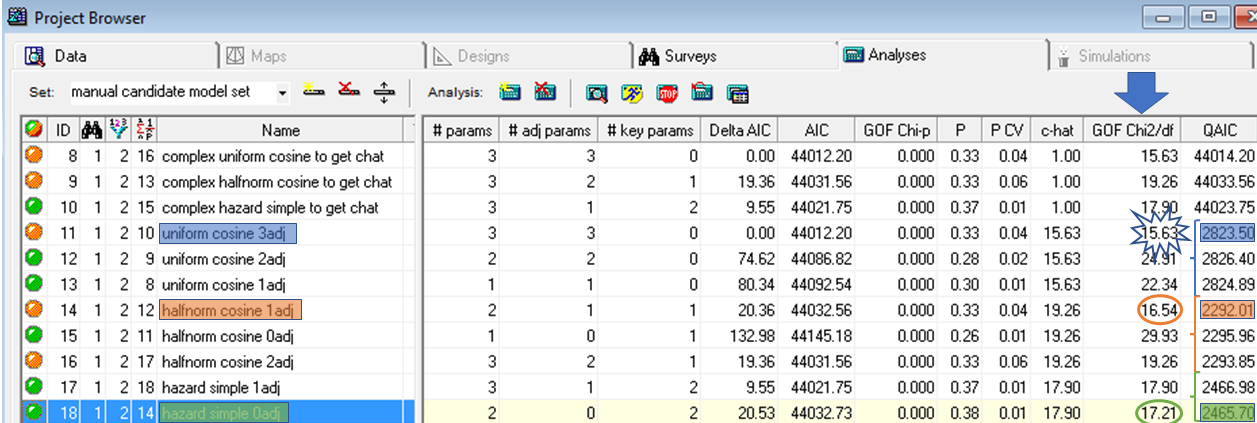
\includegraphics[width=\textwidth]{images/selection-steps-3.png}
\caption{Project browser following Step 3.  Emphasis is contrast of best models chosen from each key function family.  Compare \emph{GOF Chi2/df} values for three highlighted models.  Smallest \emph{GOF Chi2/df} value is 15.63 belonging to the uniform key function with three adjustment terms.  This will be used to make inference about density in Practical 5. \label{fig:step3}}
\end{figure} 
%\end{tcolorbox}
}
{
}

\section{Questions about this analysis}

\begin{itemize}
	\item Did the overdispersion approach lead to a different model choice than AIC selection algorithm?
\ifsolutionthenelse{%
	\begin{tcolorbox}[colback=green!5!white, colframe=green!60!black, title=Model selection choices]
	No, same model (uniform cosine with 3 adjustment terms) chosen from both approaches. 
\end{tcolorbox}
}
{
}
	\item How large is the difference in $\hat{P}$ estimates between the preferred model and the second preferred model?
\ifsolutionthenelse{%
	\begin{tcolorbox}[colback=green!5!white, colframe=green!60!black, title=Differences in $\hat{P}$]
		The estimates are identical to two decimal places ($\hat{P}$=0.33)
		\end{tcolorbox}
}
{
}
\end{itemize}

\printbibliography

\end{document}